% questions.tex —— 2006 年·四川卷·理科 · 题目内容片段（无答案）
% 由 tools/generate_projects.py 依来源总账自 2006/2006_数学真题_四川理_试题.md 生成，勿手改（改源 MD 后重跑）


\begin{gktip}
\textbf{来源边界}：题签依据固定 PDF 首页照录。题面按固定 PDF 第1—2页转录，印刷页码为332—333。固定副本的发布者、出版者、版次、来源链及官方身份均未核；\texttt{ready} 仅为来源清单中的文件状态，不代表来源认证。固定 PDF 可见范围未见答案、解析、评分或总分。
\end{gktip}

\gkpart{一、选择题}

\begin{question}
\gkti{1}已知集合 $A=\{x\mid x^2-5x+6\leqslant0\}$，集合 $B=\{x\mid |2x-1|>3\}$，则集合 $A\cap B=$\mbox{（　　）}。

（A）$\{x\mid 2\leqslant x\leqslant3\}$　　（B）$\{x\mid 2\leqslant x<3\}$

（C）$\{x\mid 2<x\leqslant3\}$　　（D）$\{x\mid -1<x<3\}$

\end{question}
\begin{question}
\gkti{2}复数 $(1-i)^3$ 的虚部为\mbox{（　　）}。

（A）$3$　　（B）$-3$　　（C）$2$　　（D）$-2$

\end{question}
\begin{question}
\gkti{3}已知
\nopagebreak[4]
\[
f(x)=
\begin{cases}
2x+3,&x\ne1,\\
2,&x=1,
\end{cases}
\]
下面结论正确的是\mbox{（　　）}。

（A）$f(x)$ 在 $x=1$ 处连续　　（B）$f(1)=5$

（C）$\displaystyle\lim_{x\to1^-}f(x)=2$　　（D）$\displaystyle\lim_{x\to1^+}f(x)=5$

\end{question}
\begin{question}
\gkti{4}已知二面角 $\alpha-l-\beta$ 的大小为 $60^\circ$，$m,n$ 为异面直线，且 $m\perp\alpha$，$n\perp\beta$，则 $m,n$ 所成的角为\mbox{（　　）}。

（A）$30^\circ$　　（B）$60^\circ$　　（C）$90^\circ$　　（D）$120^\circ$

\Needspace{0.4\textheight}
\end{question}
\begin{question}
\gkti{5}下列函数中，图象的一部分如图所示的是\mbox{（　　）}。
\nopagebreak[4]
\begin{center}% 2006 四川理科 Q5：按印刷页332题图重用同源三角函数曲线。
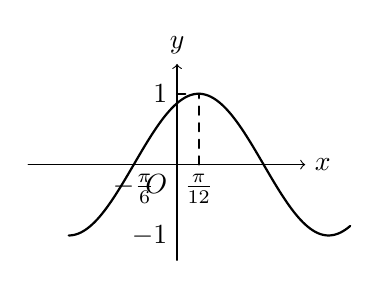
\begin{tikzpicture}[line cap=round,line join=round,x=1.05cm,y=0.9cm]
  \draw[->] (-1.8,0)--(1.55,0) node[right] {$x$};
  \draw[->] (0,-1.35)--(0,1.42) node[above] {$y$};
  \draw[thick,dashed] ({pi/12},0)--({pi/12},1);
  \draw[thick,dashed] (0,1)--({pi/12},1);
  \draw[thick,domain=-75:120,samples=120,variable=\t]
    plot ({\t*pi/180},{cos(2*\t-30)});
  \node[below left] at (0,0) {$O$};
  \node[left] at (0,1) {$1$};
  \node[left] at (0,-1) {$-1$};
  \node[below] at ({-pi/6},0) {$-\frac{\pi}{6}$};
  \node[below] at ({pi/12},0) {$\frac{\pi}{12}$};
\end{tikzpicture}
\end{center}
\nopagebreak[4]
（A）$y=\sin\left(x+\dfrac\pi6\right)$　　（B）$y=\sin\left(2x-\dfrac\pi6\right)$

（C）$y=\cos\left(4x-\dfrac\pi3\right)$　　（D）$y=\cos\left(2x-\dfrac\pi6\right)$

\end{question}
\begin{question}
\gkti{6}已知两定点 $A(-2,0)$、$B(1,0)$，如果动点 $P$ 满足 $|PA|=2|PB|$，则点 $P$ 的轨迹所包围的图形的面积等于\mbox{（　　）}。

（A）$\pi$　　（B）$4\pi$　　（C）$8\pi$　　（D）$9\pi$

\Needspace{0.4\textheight}
\end{question}
\begin{question}
\gkti{7}如图，已知正六边形 $P_1P_2P_3P_4P_5P_6$，下列向量的数量积中最大的是\mbox{（　　）}。
\nopagebreak[4]
\begin{center}% 2006 四川理科 Q7：正六边形顶点顺序与印刷页332一致。
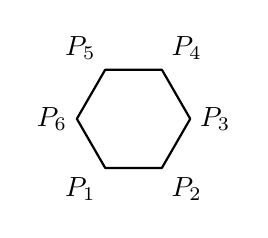
\begin{tikzpicture}[line cap=round,line join=round,x=0.72cm,y=0.72cm]
  \coordinate (P1) at (0,0);
  \coordinate (P2) at (1,0);
  \coordinate (P3) at (1.5,0.866);
  \coordinate (P4) at (1,1.732);
  \coordinate (P5) at (0,1.732);
  \coordinate (P6) at (-0.5,0.866);
  \draw[thick] (P1)--(P2)--(P3)--(P4)--(P5)--(P6)--cycle;
  \node[below left] at (P1) {$P_1$};
  \node[below right] at (P2) {$P_2$};
  \node[right] at (P3) {$P_3$};
  \node[above right] at (P4) {$P_4$};
  \node[above left] at (P5) {$P_5$};
  \node[left] at (P6) {$P_6$};
\end{tikzpicture}
\end{center}
\nopagebreak[4]
（A）$\overrightarrow{P_1P_2}\cdot\overrightarrow{P_1P_3}$　　（B）$\overrightarrow{P_1P_2}\cdot\overrightarrow{P_1P_4}$

（C）$\overrightarrow{P_1P_2}\cdot\overrightarrow{P_1P_5}$　　（D）$\overrightarrow{P_1P_2}\cdot\overrightarrow{P_1P_6}$

\end{question}
\begin{question}
\gkti{8}某厂生产甲产品每千克需用原料 $A$ 和原料 $B$ 分别为 $a_1\text{、}b_1$ 千克，生产乙产品每千克需用原料 $A$ 和原料 $B$ 分别为 $a_2\text{、}b_2$ 千克。甲、乙产品每千克可获利润分别为 $d_1\text{、}d_2$ 元。月初一次性购进本月用原料 $A\text{、}B$ 各 $c_1\text{、}c_2$ 千克。要计划本月生产甲产品和乙产品各多少千克才能使月利润总额达到最大。在这个问题中，设全月生产甲、乙两种产品分别为 $x$ 千克、$y$ 千克，月利润总额为 $z$ 元，那么，用于求使总利润 $z=d_1x+d_2y$ 最大的数学模型中，约束条件为\mbox{（　　）}。

（A）$\begin{cases}a_1x+a_2y\geqslant c_1,\\b_1x+b_2y\geqslant c_2,\\x\geqslant0,\\y\geqslant0\end{cases}$　　（B）$\begin{cases}a_1x+b_1y\leqslant c_1,\\a_2x+b_2y\leqslant c_2,\\x\geqslant0,\\y\geqslant0\end{cases}$

（C）$\begin{cases}a_1x+a_2y\leqslant c_1,\\b_1x+b_2y\leqslant c_2,\\x\geqslant0,\\y\geqslant0\end{cases}$　　（D）$\begin{cases}a_1x+a_2y=c_1,\\b_1x+b_2y=c_2,\\x\geqslant0,\\y\geqslant0\end{cases}$

\end{question}
\begin{question}
\gkti{9}直线 $y=x-3$ 与抛物线 $y^2=4x$ 交于 $A\text{、}B$ 两点，过 $A\text{、}B$ 两点向抛物线的准线作垂线，垂足分别为 $P\text{、}Q$，则梯形 $APQB$ 的面积为\mbox{（　　）}。

（A）$48$　　（B）$56$　　（C）$64$　　（D）$72$

\end{question}
\begin{question}
\gkti{10}已知球 $O$ 的半径是 $1$，$A\text{、}B\text{、}C$ 三点都在球面上，$A\text{、}B$ 两点和 $A\text{、}C$ 两点的球面距离都是 $\dfrac\pi4$，$B\text{、}C$ 两点的球面距离是 $\dfrac\pi3$，则二面角 $B-OA-C$ 的大小是\mbox{（　　）}。

（A）$\dfrac\pi4$　　（B）$\dfrac\pi3$　　（C）$\dfrac\pi2$　　（D）$\dfrac{2\pi}3$

\end{question}
\begin{question}
\gkti{11}设 $a\text{、}b\text{、}c$ 分别是 $\triangle ABC$ 的三个内角 $A\text{、}B\text{、}C$ 所对的边，则 $a^2=b(b+c)$ 是 $A=2B$ 的\mbox{（　　）}。

（A）充要条件　　（B）充分而不必要条件　　（C）必要而不充分条件　　（D）既不充分也不必要条件

\end{question}
\begin{question}
\gkti{12}从 $0$ 到 $9$ 这 $10$ 个数字中任取 $3$ 个数字组成一个没有重复数字的三位数，这个数不能被 $3$ 整除的概率为\mbox{（　　）}。

（A）$\dfrac{19}{54}$　　（B）$\dfrac{35}{54}$　　（C）$\dfrac{38}{54}$　　（D）$\dfrac{41}{60}$

\end{question}
\gkpart{二、填空题}

\begin{question}
\gkti{13}在三棱锥 $O-ABC$ 中，三条棱 $OA\text{、}OB\text{、}OC$ 两两互相垂直，且 $OA=OB=OC$，$M$ 是 $AB$ 边的中点，则 $OM$ 与平面 $ABC$ 所成角的大小是\gkblank{}。（用反三角函数表示）

\end{question}
\begin{question}
\gkti{14}设离散型随机变量 $\xi$ 可能取的值为 $1\text{、}2\text{、}3\text{、}4$，$P(\xi=k)=ak+b\ (k=1\text{、}2\text{、}3\text{、}4)$。又 $\xi$ 的数学期望 $E\xi=3$，则 $a+b=$\gkblank{}。

\Needspace{0.4\textheight}
\end{question}
\begin{question}
\gkti{15}如图，把椭圆 $\dfrac{x^2}{25}+\dfrac{y^2}{16}=1$ 的长轴 $AB$ 分成 $8$ 等分，过每个分点作 $x$ 轴的垂线交椭圆的上半部分于 $P_1\text{、}P_2\text{、}\cdots\text{、}P_7$ 七个点，$F$ 是椭圆的一个焦点，则 $|P_1F|+|P_2F|+\cdots+|P_7F|=$\gkblank{}。
\nopagebreak[4]
\begin{center}% 2006 四川理科 Q15：椭圆长轴八等分、七个上半弧点与焦点。
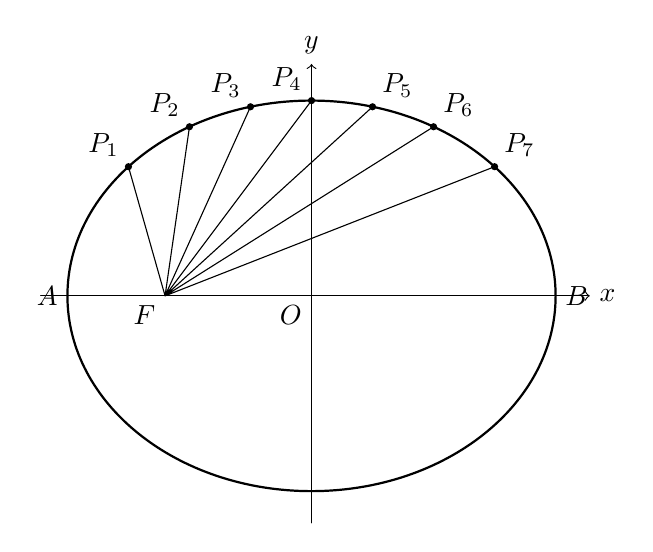
\begin{tikzpicture}[line cap=round,line join=round,x=0.62cm,y=0.62cm]
  \coordinate (P1) at (-3.75,2.646);
  \coordinate (P2) at (-2.50,3.464);
  \coordinate (P3) at (-1.25,3.873);
  \coordinate (P4) at (0,4);
  \coordinate (P5) at (1.25,3.873);
  \coordinate (P6) at (2.50,3.464);
  \coordinate (P7) at (3.75,2.646);
  \coordinate (F) at (-3,0);
  \draw[->] (-5.55,0)--(5.7,0) node[right] {$x$};
  \draw[->] (0,-4.65)--(0,4.75) node[above] {$y$};
  \draw[thick] (0,0) ellipse (5 and 4);
  \draw[thin] (F)--(P1) (F)--(P2) (F)--(P3) (F)--(P4)
              (F)--(P5) (F)--(P6) (F)--(P7);
  \foreach \i in {1,...,7} \fill (P\i) circle (1.3pt);
  \node[left] at (-5,0) {$A$};
  \node[right] at (5,0) {$B$};
  \node[below left] at (F) {$F$};
  \node[below left] at (0,0) {$O$};
  \node[above left] at (P1) {$P_1$};
  \node[above left] at (P2) {$P_2$};
  \node[above left] at (P3) {$P_3$};
  \node[above left] at (P4) {$P_4$};
  \node[above right] at (P5) {$P_5$};
  \node[above right] at (P6) {$P_6$};
  \node[above right] at (P7) {$P_7$};
\end{tikzpicture}
\end{center}
\nopagebreak[4]
\end{question}
\gkpart{三、解答题}

\begin{question}
\gkti{16}非空集合 $G$ 关于运算 $\oplus$ 满足：(1) 对任意 $a\text{、}b\in G$，都有 $a\oplus b\in G$；(2) 存在 $e\in G$，使得对一切 $a\in G$，都有 $a\oplus e=e\oplus a=a$，则称 $G$ 关于运算 $\oplus$ 为“融洽集”。现给出下列集合和运算：

① $G=\{\text{\text{非负整数}}\}$，$\oplus$ 为整数的加法；

② $G=\{\text{\text{偶数}}\}$，$\oplus$ 为整数的乘法；

③ $G=\{\text{\text{平面向量}}\}$，$\oplus$ 为平面向量的加法；

④ $G=\{\text{\text{二次三项式}}\}$，$\oplus$ 为多项式的加法；

⑤ $G=\{\text{\text{虚数}}\}$，$\oplus$ 为复数的乘法。

其中 $G$ 关于运算 $\oplus$ 为“融洽集”的是\gkblank{}。（写出所有“融洽集”的序号）

\end{question}
\begin{question}
\gkti{17}已知 $A\text{、}B\text{、}C$ 是 $\triangle ABC$ 三内角，向量 $\mathbf m=(-1,\sqrt3)$、$\mathbf n=(\cos A,\sin A)$，且 $\mathbf m\cdot\mathbf n=1$。

(1) 求角 $A$；

(2) 若 $\dfrac{1+\sin2B}{\cos^2B-\sin^2B}=-3$，求 $\tan C$。

\end{question}
\begin{question}
\gkti{18}某课程考核分理论和实验两部分进行，每部分考核成绩只记“合格”与“不合格”，两部分考核都“合格”则该课程考核“合格”。甲、乙、丙三人在理论考核中合格的概率分别为 $0.9\text{、}0.8\text{、}0.7$；在实验考核中合格的概率分别为 $0.8\text{、}0.7\text{、}0.9$。所有考核是否合格互相之间没有影响。

(1) 求甲、乙、丙三人在理论考核中至少有两人合格的概率；

(2) 求这三人该课程考核都合格的概率。（结果保留三位小数）

\Needspace{0.4\textheight}
\end{question}
\begin{question}
\gkti{19}如图，在长方体 $ABCD-A_1B_1C_1D_1$ 中，$E\text{、}P$ 分别是 $BC\text{、}A_1D_1$ 的中点，$M\text{、}N$ 分别是 $AE\text{、}CD_1$ 的中点，$AD=AA_1=a$，$AB=2a$。

(1) 求证：$MN\parallel$ 面 $ADD_1A_1$；

(2) 求二面角 $P-AE-D$ 的大小；

(3) 求三棱锥 $P-DEN$ 的体积。
\nopagebreak[4]
\begin{center}% 2006 四川理科 19：长方体 ABCD-A_1B_1C_1D_1 及题设中点、构造线
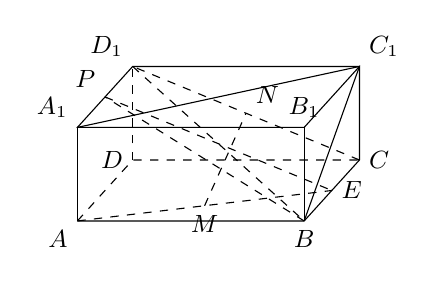
\begin{tikzpicture}[scale=0.9, font=\small]
  % 斜投影：AB=2a，AD=AA_1=a；比例仅用于示意。
  \coordinate (A)  at (0,0);
  \coordinate (B)  at (3.2,0);
  \coordinate (D)  at (0.78,0.86);
  \coordinate (C)  at (3.98,0.86);
  \coordinate (A1) at (0,1.32);
  \coordinate (B1) at (3.2,1.32);
  \coordinate (D1) at (0.78,2.18);
  \coordinate (C1) at (3.98,2.18);
  \coordinate (E)  at (3.59,0.43);
  \coordinate (P)  at (0.39,1.75);
  \coordinate (M)  at (1.795,0.215);
  \coordinate (N)  at (2.38,1.52);

  % 实线棱：前面、右侧及上部可见轮廓。
  \draw (A)--(B)--(C)--(C1)--(B1)--(A1)--(D1)--(C1);
  \draw (A)--(A1);
  \draw (B)--(B1);
  % 题图中的辅助线。
  \draw (A1)--(C1);
  \draw (B)--(C1);

  % 被遮挡的棱与位于后方/底面的构造线。
  \draw[dashed] (A)--(D)--(C);
  \draw[dashed] (D)--(D1);
  \draw[dashed] (A)--(E);
  \draw[dashed] (M)--(N);
  \draw[dashed] (P)--(E);
  \draw[dashed] (B)--(P);
  \draw[dashed] (D1)--(B);
  \draw[dashed] (C)--(D1);

  \node[below left] at (A) {$A$};
  \node[below] at (B) {$B$};
  \node[right] at (C) {$C$};
  \node[left] at (D) {$D$};
  \node[above left] at (A1) {$A_1$};
  \node[above] at (B1) {$B_1$};
  \node[above right] at (C1) {$C_1$};
  \node[above left] at (D1) {$D_1$};
  \node[above left] at (P) {$P$};
  \node[above right] at (N) {$N$};
  \node[below] at (M) {$M$};
  \node[right] at (E) {$E$};
\end{tikzpicture}
\end{center}
\nopagebreak[4]
\end{question}
\begin{question}
\gkti{20}已知数列 $\{a_n\}$，其中 $a_1=1$，$a_2=3$，$2a_n=a_{n+1}+a_{n-1}\ (n\geqslant2)$。记数列 $\{a_n\}$ 的前 $n$ 项和为 $S_n$，数列 $\{\ln S_n\}$ 的前 $n$ 项和为 $U_n$。

(1) 求 $U_n$；

\Needspace{5\baselineskip}
(2) 设
\nopagebreak[4]
\[
F_n(x)=\frac{e^{U_n}}{2n(n!)^2}x^{2n}\quad(x>0),\qquad
T_n(x)=\sum_{k=1}^{n}F'_k(x)
\]
\Needspace{5\baselineskip}
（其中 $F'_k(x)$ 为 $F_k(x)$ 的导函数），计算
\nopagebreak[4]
\[
\lim_{n\to\infty}\frac{T_n(x)}{T_{n+1}(x)}\mbox{。}
\]

\end{question}
\begin{question}
\gkti{21}已知两定点 $F_1(-\sqrt2,0)\text{、}F_2(\sqrt2,0)$，满足条件 $|\overrightarrow{PF_2}|-|\overrightarrow{PF_1}|=2$ 的点 $P$ 的轨迹是曲线 $E$，直线 $y=kx-1$ 与曲线 $E$ 交于 $A\text{、}B$ 两点。如果 $|\overrightarrow{AB}|=6\sqrt3$，且曲线 $E$ 上存在点 $C$，使 $\overrightarrow{OA}+\overrightarrow{OB}=m\overrightarrow{OC}$，求 $m$ 的值和 $\triangle ABC$ 的面积 $S$。

\end{question}
\begin{question}
\gkti{22}已知函数 $f(x)=x^2+\dfrac2x+a\ln x\ (x>0)$，$f(x)$ 的导函数是 $f'(x)$。对任意两个不相等的正数 $x_1\text{、}x_2$，证明：

\Needspace{5\baselineskip}
(1) 当 $a\leqslant0$ 时，
\nopagebreak[4]
\[
\frac{f(x_1)+f(x_2)}2>f\left(\frac{x_1+x_2}2\right);
\]

\Needspace{5\baselineskip}
(2) 当 $a\leqslant4$ 时，
\nopagebreak[4]
\[
|f'(x_1)-f'(x_2)|>|x_1-x_2|\mbox{。}
\]

\end{question}